\documentclass[12pt,english]{article}
\usepackage[a4paper,bindingoffset=0.2in,%
            left=1in,right=1in,top=1in,bottom=1in,%
            footskip=.25in]{geometry}
\usepackage{blindtext}
\usepackage{titling}
\usepackage{amssymb}
\usepackage{listofitems,amsmath}
\usepackage{listings}
\usepackage{lettrine} 
\usepackage{tikz}  
\usepackage{color} 
\usepackage{xcolor}
\usetikzlibrary{shapes, arrows, calc, arrows.meta, fit, positioning} % these are the parameters passed to the library to create the node graphs  
\tikzset{>=latex} % for LaTeX arrow head
\tikzset{  
    -Latex,auto,node distance =0.6 cm and 1.3 cm, thick,% node distance is the distance between one node to other, where 1.5cm is the length of the edge between the nodes  
    state/.style ={ellipse, draw, minimum width = 0.9 cm}, % the minimum width is the width of the ellipse, which is the size of the shape of vertex in the node graph  
    point/.style = {circle, draw, inner sep=0.18cm, fill, node contents={}},  
    bidirected/.style={Latex-Latex,dashed}, % it is the edge having two directions  
    el/.style = {inner sep=2.5pt, align=right, sloped}  
}  
\colorlet{mydarkblue}{blue!40!black}
\tikzstyle{connect}=[thick,mydarkblue] %,line cap=round
\tikzstyle{connect arrow}=[-{Latex[length=4,width=3.5]},thick,mydarkblue,shorten <=0.5,shorten >=1]
\usepackage[outline]{contour} % glow around text
\setlength{\parskip}{12pt}
\title{Home Work 6 Undergraduate}
\date{\today}
\author{Jose Carlos Munoz}
%================================
\begin{document}
\newgeometry{left=0.8in,right=0.8in,top=1in,bottom=1in}
\begin{center}
    \Large
    \textbf{Homework 6}\\
    \small
    \today\\
    \large
    Jose Carlos Munoz
\end{center}
%===============================
\section*{1}
The RNN would most likely suffer from vanishin gradient. While the transformation of the function is 3.5, the derivative of the sigmoid activation is always less than 0.25. When doing back propogation, the value between these numbers is less than 1. So , in a Recurrent network, it will be dramatically go small. So this RNN will suffer from vanishing gadient.
\section*{2}
The rule is that spectral radius times the activation function highest value to be as close to one. Since, we know that the value can blow up 8 times high, we can set the spectral radius to a $\frac{1}{8}$. So that they both multiply to be at most 1
\section*{3}
The computation graph of the RNN cell is as follows
% Input layer neurons'number
\newcommand{\inputnum}{2}  
% Hidden layer neurons'number
\newcommand{\hiddennum}{2}   
% Output layer neurons'number
\newcommand{\outputnum}{1} 
\begin{figure}[htb]
\begin{center}
\resizebox{1\textwidth}{!}{
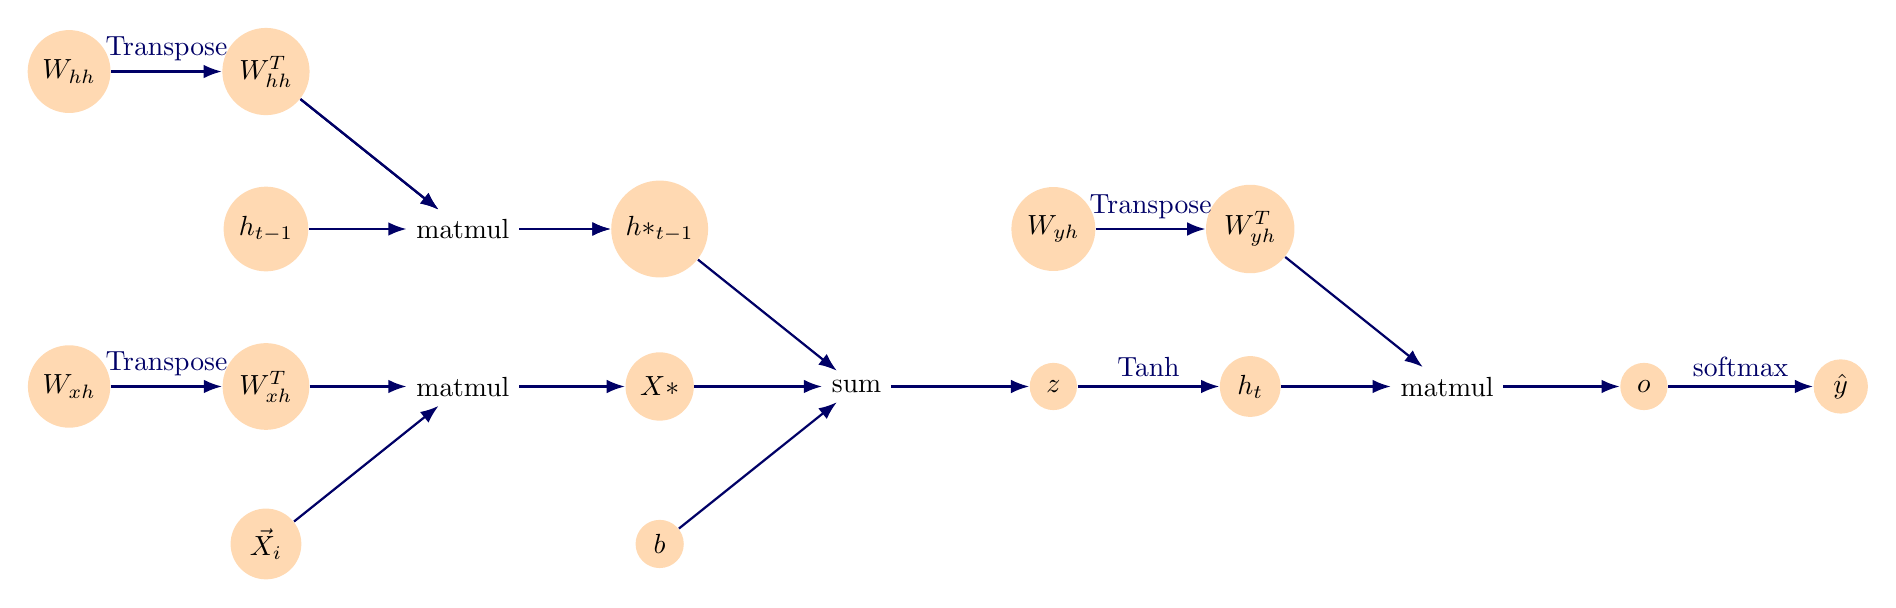
\begin{tikzpicture} 
\node[circle,  minimum size = 6mm, fill=orange!30] (ht1) at (2.5, -2) {$h_{t-1}$};\node[circle,  minimum size = 6mm, fill=orange!30] (ht1p) at (7.5,-2) {$h*_{t-1}$};\node[circle,  minimum size = 6mm, fill=orange!30] (wyh) at (12.5, -2) {$W_{yh}$};\node[circle,  minimum size = 6mm, fill=orange!30] (wyht) at (15,-2) {$W_{yh}^{T}$};
\node[circle,  minimum size = 6mm, fill=orange!30] (whh) at (0,0) {$W_{hh}$};\node[circle,  minimum size = 6mm, fill=orange!30] (whht) at (2.5,0) {$W_{hh}^{T}$};
\node[circle,  minimum size = 6mm, fill=orange!30] (wxh) at (0,-4) {$W_{xh}$};\node[circle,  minimum size = 6mm, fill=orange!30] (wxht) at (2.5,-4) {$W_{xh}^{T}$};\node[circle,  minimum size = 6mm, fill=orange!30] (xp) at (7.5,-4) {$X*$};\node[circle,  minimum size = 6mm, fill=orange!30] (z) at (12.5,-4) {$z$};\node[circle,  minimum size = 6mm, fill=orange!30] (h) at (15,-4) {$h_{t}$};\node[circle,  minimum size = 6mm, fill=orange!30] (o) at (20,-4) {$o$};\node[circle,  minimum size = 6mm, fill=orange!30] (y) at (22.5,-4) {$\hat{y}$};
\node[circle,  minimum size = 6mm, fill=orange!30] (x) at (2.5,-6) {$\vec{X}_{i}$};\node[circle,  minimum size = 6mm, fill=orange!30] (b) at (7.5,-6) {$b$};

\node (1) at (5,-2) {matmul};
\node (2) at (5,-4) {matmul};
\node (3) at (10,-4) {sum};
\node (4) at (17.5,-4) {matmul};

\draw[connect](whh)--(whht)node[pos=0.5]{Transpose};\draw[connect](wxh)--(wxht)node[pos=0.5]{Transpose};\draw[connect](wyh)--(wyht)node[pos=0.5]{Transpose};
\draw[connect](o)--(y)node[pos=0.5]{softmax};
\draw[connect](whht)--(1);\draw[connect](ht1)--(1);\draw[connect](whht)--(1);\draw[connect](1)--(ht1p);
\draw[connect](wxht)--(2);\draw[connect](x)--(2);\draw[connect](2)--(xp);\draw[connect](1)--(ht1p);
\draw[connect](ht1p)--(3);\draw[connect](xp)--(3);\draw[connect](3)--(z);\draw[connect](b)--(3);
\draw[connect](z)--(h)node[pos=0.5]{Tanh};
\draw[connect](wyht)--(4);\draw[connect](h)--(4);\draw[connect](4)--(o);
\end{tikzpicture}
}
\end{center}
 \end{figure}
\end{document}
